\chapter{Matched-law detection studies}
\label{ch:synthetic}

This chapter reports what the matched synthetic studies establish about detecting marked stress sensitivity when parts of the background and triggering process are estimated. The historical comparisons below concern their stated law class and finite numerical implementation; the subsequent F continuation is reported separately at the end of the chapter. The common alternative bank contains \(150\) stronger histories, and each procedure has \(1{,}000\) null queries with \(999\) separately identified null references. Success is a calibrated rejection on an alternative history; the null rejection rate counts rejections among uninhibited query histories. Figure~\ref{fig:detection} summarizes the detection rates and their conditional binomial intervals.

\begin{table}[tbp]
\centering
\caption{Historical detection on the common stronger alternative bank and null rejection on \(1{,}000\) null queries. Intervals are nominal \(95\%\) Clopper--Pearson intervals conditional on the fixed bank and law.}
\label{tab:main-detection}
\small
\setlength{\tabcolsep}{4pt}
\begin{tabular}{@{}p{0.40\linewidth}ccc@{}}
\toprule
Procedure & Detections & \(95\%\) interval & Null rejections \\
\midrule
Known laws (fixed \(\eta\)) & \(150/150\) & \(97.57\)--\(100\%\) & \(50/1000\) \\
\(\eta\) estimated; nuisances supplied & \(150/150\) & \(97.57\)--\(100\%\) & \(49/1000\) \\
Level estimated; trend supplied & \(123/150\) & \(74.90\)--\(87.79\%\) & \(46/1000\) \\
Level and trend estimated & \(68/150\) & \(37.20\)--\(53.66\%\) & \(44/1000\) \\
Historical fuller fitted procedure & \(57/150\) & \(30.21\)--\(46.28\%\) & \(50/1000\) \\
\bottomrule
\end{tabular}
\end{table}

For the first four procedures, the triggering process, mark exponent \(\beta\), and both kernels are supplied. The first row supplies both laws completely. The second estimates \(\eta\) while supplying the remaining nuisance values. The third estimates \(\eta\) and background level while supplying the trend, and the fourth estimates \(\eta\), background level and trend. The final row is the fuller historical fitted procedure, which additionally estimates or searches the triggering, mark, and kernel components under the earlier recipe. It is therefore not a purely nested extension of the fourth row, and its count should not be interpreted as an independent replication.

The known-laws (fixed \(\eta\)) procedure detects every one of the \(150\) stronger alternatives. This demonstrates that, for the evaluated generating law and numerical kernels, the stronger marked sensitivity is distinguishable when the comparison laws are supplied. It is not a statement of intrinsic inability to distinguish arbitrary physical mechanisms, nor a proof that all mechanisms would be easy to distinguish in observed data. The \(\eta\)-estimated, nuisances-supplied procedure also detects all \(150\). There is no observed loss from estimating that parameter alone on this bank; this does not prove equality of population detection probabilities. Estimating the background level leaves \(123\) detections, while estimating both level and trend leaves \(68\). These named-procedure differences are not an additive attribution of the gap. Moving from \(150\) to \(123\) and from \(123\) to \(68\) describes the tested configurations; it does not decompose the loss into independently estimable physical or numerical contributions.

The realized null rates lie between \(4.4\%\) and \(5.0\%\). In row order, the conditional \(95\%\) null intervals are \(3.73\)--\(6.54\%\), \(3.65\)--\(6.43\%\), \(3.39\)--\(6.09\%\), \(3.21\)--\(5.86\%\), and \(3.73\)--\(6.54\%\). These similar observed rates are useful calibration summaries, but they do not establish equal test size uniformly over the composite null. The intervals are conditional on the realized reference bank and law, and the procedures were selected through research reuse.


\begin{figure}[tbp]
\centering
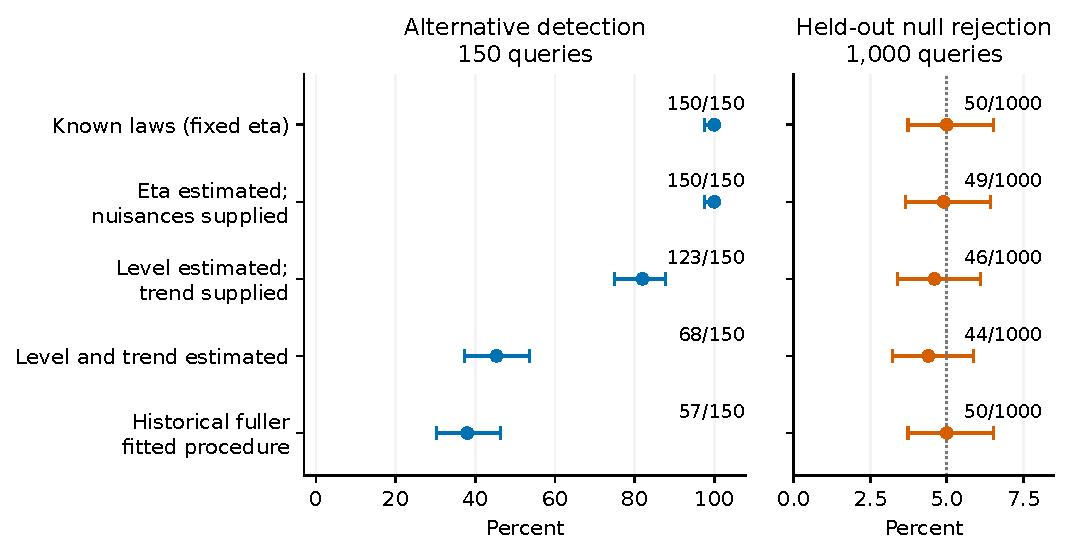
\includegraphics[width=\linewidth]{detection.pdf}
\caption{Historical matched-null detection on the same 150 stronger alternatives. Error bars are nominal conditional 95\% binomial intervals. Each procedure has its own 999 reference statistics and 1,000 separate null queries; adaptive selection and reference-bank uncertainty are omitted.}
\label{fig:detection}
\end{figure}

\section{Sensitivity to the diagnostic value}

The value of \(\eta\) changes the histories as well as the fixed-history intensity separation. In a paired comparison using the same \(150\) fresh pairs, the initial value \(\eta=0.2839974288868791\) produced \(49/150\) detections for the fuller fitted procedure, whereas the adjusted value \(\eta=0.4885010300470942\) produced \(57/150\). The paired gain is therefore \(8\) detected histories, or \(5.33\) percentage points, with a descriptive Monte Carlo standard error of \(4.71\) percentage points. A separate \(25\)-pair planning sample gave \(6/25\) and \(11/25\) under the two values; it is a planning exercise and is not pooled with the \(150\)-pair comparison.

The descriptive paired Monte Carlo standard error uses the sample variance of paired decision differences. For \(N_{\mathrm{pair}}\) pairs, let \(D_i\in\{-1,0,1\}\) be the first decision minus the second, with positive and negative discordance counts \(b,c\). Then
\[
 \overline D=\frac{b-c}{N_{\mathrm{pair}}},\qquad
 \widehat{\operatorname{MCSE}}
 =\sqrt{\frac{b+c-N_{\mathrm{pair}}\overline D^{\,2}}
 {N_{\mathrm{pair}}(N_{\mathrm{pair}}-1)}}.
\]
This is the sample standard deviation of \(D_i\) divided by \(\sqrt{N_{\mathrm{pair}}}\). Taking the adjusted-value decision first gives \(b=29,c=21\) and \(N_{\mathrm{pair}}=150\), hence \(4.7096\) percentage points, rounding to \(4.71\). Using empirical-variance divisor \(N_{\mathrm{pair}}\) instead gives a slightly different value from the same outcomes. The stated fixed-bank and adaptive-reuse qualifications still apply; no new test is added.

The mean achieved fixed-history total intensity suppression was \(14.159\%\) for the initial value and \(19.360\%\) for the adjusted value. For a realized nonempty history and fixed generating nuisance, the event-mean functional is
\begin{equation}
 S(\eta;\mathcal H_T)=\frac{100}{N_T}\sum_{i=1}^{N_T}
 \frac{B(t_i)\{1-e^{-\eta G_s(t_i)}\}}
      {B(t_i)+nH_e(t_i)}.
 \label{eq:achieved-suppression}
\end{equation}
Both intensities in each comparison use the same strictly earlier history. The reported mean then gives equal weight to each catalogue's event mean, rather than pooling every event across catalogues. This is the functional implemented in \hyperlink{S07}{archival \texttt{S07} (not distributed)}.
It is an event-mean description of separation on a common history, not a controlled reduction in earthquake count. Increasing \(\eta\) also changes the synthetic histories that are subsequently realized. Counts remain random, and no monotonicity of realized counts is guaranteed. An extreme retained pair, with \(449\) events under one member and \(6{,}553\) under the other, illustrates why suppression of a fixed-history rate cannot be reported as a promise about realized totals.

An earlier archive used a \(1{,}999\)-reference rank denominator of \(2{,}000\). The later recalibration using \(999\) references and \(1{,}000\) separate null queries produced the same count of \(57\) detections only by happenstance. It is a consistency observation, not an independent replication, and the two reference constructions should not be combined. The \href{https://github.com/Drefetr/InhibitoryEarthquakeModels/blob/3e76a174cf4f58ce601c6c9640c4d0c11168813f/paper/data/paired.json}{public paired summary} retains aggregate pairing results; the historical study is reported in \hyperlink{S08}{archival \texttt{S08} (not distributed)}. The completed-history provenance for later recalibration is recorded in \hyperlink{S09}{archival \texttt{S09} (not distributed)} and the final results in \hyperlink{S16}{archival \texttt{S16} (not distributed)}.

\section{Paired comparison of level and trend}

The level-and-trend comparison is more informative when the two procedures are paired on the same \(150\) histories rather than read only from marginal detection counts. Figure~\ref{fig:paired} crosses their decisions. Both procedures detect on \(62\) histories, the level-only procedure detects on \(61\) where the combined procedure does not, the combined procedure detects on \(6\) where level-only does not, and neither detects on \(21\). The marginal counts are therefore \(123\) and \(68\), and the difference is \(55/150=36.67\) percentage points, with a descriptive paired Monte Carlo standard error of \(4.58\) percentage points, using the same sample-variance convention with \(b=61,c=6\) and \(N_{\mathrm{pair}}=150\) (\(4.5776\) before rounding).

There is no pathwise dominance. The level-only procedure detects on \(61\) histories where the combined procedure does not, while the reverse occurs on \(6\). The \(55\)-history marginal gap is real for this realized paired bank, but the paired arrangement shows that it is not produced by a uniform improvement. Among the \(999\) null reference scores for the level-only procedure, \(604\) were exactly zero. Ties and the add-one rank rule are therefore material in that calibration. Different null thresholds can alter the comparison and must be considered when interpreting the paired decisions.

A ten-history raw-statistic pilot contained six null and four alternative histories. On that small pilot, level-only contraction exceeded trend-only contraction on four alternatives. This is a descriptive diagnostic of local score behavior, not a calibrated power comparison. That historical experiment does not contain a fully calibrated trend-only row, so the level-only discordance cannot be assigned uniquely to trend. The absence of that row does not imply that trend-only would perform best, nor does it automatically identify trend-only calibration as the best next experiment. A fair decision among procedures would require its own reference bank and calibration under the same reporting rules.

All \(1{,}150\) decisions in the reported historical detection-and-null evaluation resolved under the empirical numerical envelopes. That is a completeness statement for this realized study, not a rigorous universal bound on numerical integration or optimization. The selected-ten pilot is documented in \hyperlink{S15}{archival \texttt{S15} (not distributed)}. The paired detection table and matched-null results are documented in \hyperlink{S16}{archival \texttt{S16} (not distributed)}.


\begin{figure}[!htbp]
\centering
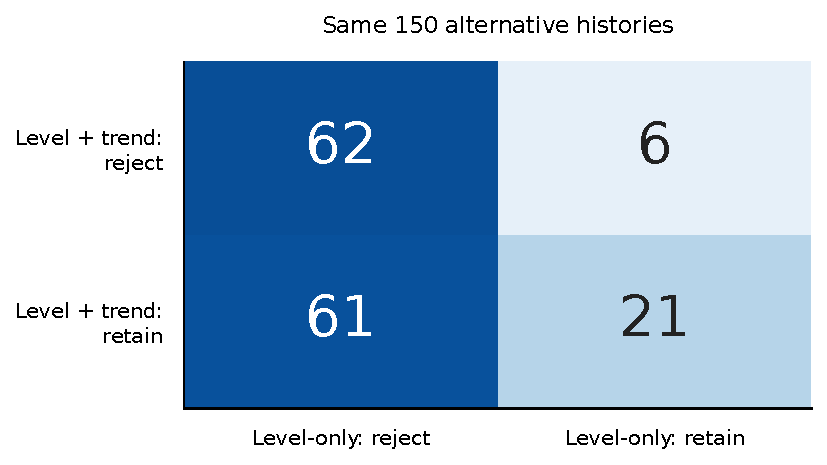
\includegraphics[width=0.68\linewidth]{paired.pdf}
\caption{Paired decisions for background level alone versus level and trend estimated. The 61 versus six discordant histories yield a 36.67 percentage-point net difference, but neither procedure dominates on every history.}
\label{fig:paired}
\end{figure}

\section{Diagnostics and limits of explanation}

A separate audit examined ten selected difficult completed histories using a larger iteration limit and a Powell search. The largest phase improvement in negative log likelihood was \(1.94995664\times10^{-8}\), and the largest direct generalized-likelihood-ratio change was \(3.89681745\times10^{-8}\), below the declared diagnostic screens of \(0.001\) for phase negative log likelihood and \(0.1\) for the direct statistic. These histories were selected because they were difficult, so the audit is neither representative of the full bank nor a global optimization guarantee. Within the audited set, however, it weakens an explanation of the fitted-law gap based on inadequate optimizer stopping. It does not eliminate the possibility of optimizer limitations on other histories. This selected-ten audit concerns the historical recipe; the later F solver diagnostics and unresolved outcomes are separately reported in the addendum.

Two pre-existing fixed-history score projections onto \(a\), \(d\), and \(n\) retain \(10.82\%\) and \(3.26\%\) of weighted \(\eta\) squared-score norms. These percentages show local overlap between the directions in which the background parameters and the diagnostic parameter move the score. They are not ensemble Fisher information, not fractions of statistical power, and not an explanation of the observed \(38\%\) fitted detection rate.

Saved likelihood accounting provides one further descriptive check: estimating background level and trend improved the selected null likelihood more than the alternative likelihood on all \(150\) histories, with median null negative-log-likelihood gain \(28.665\) versus \(0.862\) for the alternatives. This records how the supplied comparison accounted for background in these specific histories. It is not a measurement of physical loading. The optimizer audit is reported in \hyperlink{S14}{archival \texttt{S14} (not distributed)}; the score geometry is reported in \hyperlink{S02}{archival \texttt{S02} (not distributed)}; and the saved likelihood accounting is documented in \hyperlink{S11}{archival \texttt{S11} (not distributed)}.

Taken together, the matched studies locate a substantial change in calibrated detection when background parameters are estimated: under the stated synthetic law, the stronger alternatives are distinguishable with supplied laws and with \(\eta\) alone estimated, while fitting background components changes the calibrated detection outcome. The experiments cannot separate the unavoidable difficulty of a composite statistical problem from recoverable loss in a particular fitted procedure. They are controlled matched-law tests rather than empirical physical discovery, and the reported boundaries follow from that design. The scoped contribution is a reproducible, numerically explicit assessment of where the marked-sensitivity signal is retained or attenuated by estimation, together with the calibration limits needed to read it. 

The \href{https://github.com/Drefetr/InhibitoryEarthquakeModels/blob/3e76a174cf4f58ce601c6c9640c4d0c11168813f/paper/data/detection.json}{public detection summary} and the \hyperref[sec:source-supplements]{availability guide} provide public entry points. Saved summaries do not replace the omitted full authorities or historical history banks.

\section{A bounded four-procedure continuation}
\label{sec:f-continuation}

The accompanying \emph{F continuation: background nuisance estimation}
addendum (22 October 2026 revision; scientific execution on 19 October UTC)
reports a subsequent exploratory study. It uses the same pinned catalogue
and clock identities as the historical level-only and level-and-trend
studies, but fits a separately frozen finite numerical procedure with its
own mandatory solver and control rules. Every alternative estimates
\(\eta\); the background log level \(a\) and trend \(d\) are supplied or
estimated in a four-cell design. The supplied/supplied cell is therefore
distinct from the fixed-\(\eta\) known-law benchmark above.

\begin{table}[H]
\centering
\caption{Separate F continuation: decisions on all 150 planned alternative
queries at \(\alpha=0.05\). These counts belong to the new finite procedure,
not the historical table or its conditional binomial intervals.}
\label{tab:f-continuation}
\small
\begin{tabular}{@{}lrrr@{}}\toprule
Background nuisance fitted & Reject & Non-reject & Unknown\\\midrule
Neither (\(I_{00}\)) & 150 & 0 & 0\\
Level only (\(I_{10}\)) & 122 & 28 & 0\\
Trend only (\(I_{01}\)) & 150 & 0 & 0\\
Level and trend (\(I_{11}\)) & 65 & 82 & 3\\\bottomrule
\end{tabular}
\end{table}

All 2,149 identities remain registered, but only 7,068 of 8,596 planned
method outcomes have controlled statistics; 1,528 remain unknown. The
null-query rejection accounting bounds are \([0.030,0.407]\),
\([0.035,0.412]\), \([0.031,0.414]\) and \([0.031,0.411]\) in cell order,
using all 1,000 planned null queries. These are missing-decision bounds,
not confidence intervals. History cost, traversal and stopping rules make
missingness nonrandom. The continuation has not established its empirical
null size, and its alternative rejection fractions do not establish a
size-matched power ranking. Its full-pair interaction point mean and MCSE
remain unavailable. All 2,000 descriptive shared-reference/paired-query
resamples completed; their endpoint quantiles do not supply certified coverage.

A posthoc lineage check within the continuation fixed its original
25-query pilot cohort. The same level-only query fits and statistics gave
6 definite rejections, 11 non-rejections and 8 unknowns under the pilot
reference calibration, then 19, 6 and 0 under the expanded calibration.
This is calibration-dependent decision accounting. That 25-query cohort
is distinct from the earlier 25-pair \(\eta\)-planning sample reported
above. Neither comparison is an independent replication.

The trend-only cell now provides a bounded comparison under the new
procedure; it does not retrospectively explain the historical level-only
discordance. The addendum retains partial geometry diagnostics, failures,
methods and availability limits. The results support sensitivity to the
specified nuisance and calibration treatment, without identifying an
unavoidable loss, a physical mechanism or a universal benefit from a
particular nuisance restriction. The historical counts, intervals and
figures above remain results of their original recipes and are not pooled
with or overwritten by this continuation.

